%====================================================================%
%                  MORIOND.TEX                                       %
% This latex file rewritten from various sources for use in the      %
% preparation of the standard proceedings Volume, latest version     %
% for the Neutrino'96 Helsinki conference proceedings                %
% by Susan Hezlet with acknowledgments to Lukas Nellen.              %
% Some changes are due to David Cassel.                              %
%====================================================================%

%\documentstyle[11pt,moriond,epsfig]{article}
\documentclass[11pt]{article}
\usepackage{moriond,epsfig}
\usepackage{xspace}

\bibliographystyle{unsrt}    
% for BibTeX - sorted numerical labels by order of
% first citation.

% A useful Journal macro
\def\Journal#1#2#3#4{{#1} {\bf #2}, #3 (#4)}

% Some useful journal names
\def\NCA{\em Nuovo Cimento}
\def\NIM{\em Nucl. Instrum. Methods}
\def\NIMA{{\em Nucl. Instrum. Methods}~A}
\def\NPB{{\em Nucl. Phys.}~B}
\def\PLB{{\em Phys. Lett.}~B}
\def\PRL{\em Phys. Rev. Lett.}
\def\PRD{{\em Phys. Rev.}~D}
\def\ZPC{{\em Z. Phys.}~C}
\def\JINST{{\em JINST} }
\def\JHEP{{\em JHEP} }

% Some other macros used in the sample text
\def\st{\scriptstyle}
\def\sst{\scriptscriptstyle}
\def\mco{\multicolumn}
\def\epp{\epsilon^{\prime}}
\def\vep{\varepsilon}
\def\ra{\rightarrow}
\def\ppg{\pi^+\pi^-\gamma}
\def\vp{{\bf p}}
\def\ko{K^0}
\def\kb{\bar{K^0}}
\def\al{\alpha}
\def\ab{\bar{\alpha}}
\def\be{\begin{equation}}
\def\ee{\end{equation}}
\def\bea{\begin{eqnarray}}
\def\eea{\end{eqnarray}}
\def\CPbar{\hbox{{\rm CP}\hskip-1.80em{/}}}
%temp replacement due to no font

\def\GeVmass {GeV\xspace}
\def\GeVmom {GeV\xspace}
\def\sqrts {$\sqrt{s}=7$~TeV\xspace}
\def\etmiss {\ensuremath{E_{\mathrm{T}}\hspace{-1.1em}/\kern0.5em}\xspace}
\def\pt{\ensuremath{p_{\rm T}}\xspace}
\def\pp{proton-proton\xspace}
\def\Zprime{Z\`\xspace}
\def\Wprime{W\`\xspace}
\def\gravitonKK{$\rm{G}_{\rm{KK}}$\xspace}

%%%%%%%%%%%%%%%%%%%%%%%%%%%%%%%%%%%%%%%%%%%%%%%%%%
%                                                %
%    BEGINNING OF TEXT                           %
%                                                %
%%%%%%%%%%%%%%%%%%%%%%%%%%%%%%%%%%%%%%%%%%%%%%%%%%
\begin{document}
\vspace*{4cm}
\title{EXOTICA SEARCHES AT THE CMS EXPERIMENT}

\author{F. SANTANASTASIO \\(ON BEHALF OF THE CMS COLLABORATION)}

\address{University of Maryland, Department of Physics - John S. Toll Physics Building, \\ College Park, MD 20742-4111, United States of America}

\maketitle\abstracts{
This paper presents the results of searches for various new physics 
phenomena in proton-proton collisions at $\sqrt{s}=7$~TeV delivered 
by the LHC and collected with the CMS detector in 2010. 
While the sensitivity of these early searches varies, 
in many cases they set the most stringent limits on these 
new physics phenomena. These results demonstrate good understanding 
of the detector and backgrounds in a variety of channels, 
which is a fundamental component of successful searches in view 
of the much larger data sample expected to be delivered by LHC in 2011 and beyond.
%% This is where the abstract should be placed. It should consist of one paragraph
%% and give a concise summary of the material in the article below.
%% Replace the title, authors, and addresses within the curly brackets
%% with your own title, authors, and addresses; please use
%% capital letters for the title and the authors. You may have as many authors and
%% addresses as you wish. It's preferable not to use footnotes in the abstract
%% or the title; the
%% acknowledgments for funding bodies etc. are placed in a separate section at
%% the end of the text.
}

\section{Introduction}
The standard model (SM) of particle physics has been extremely
successful in describing all phenomena at the highest 
attainable energies thus far. Yet, it is widely believed 
to be only an effective description of a more complete theory, 
which supersedes it at higher energy scales. Many theoretical 
extensions of the SM have been proposed in the past decades, 
which usually predict the existence of new particles. Examples 
of such conjectured particles are the \Zprime and \Wprime bosons, 
fourth-generation fermions, supersymmetric particles, leptoquarks, 
excited quarks, gravitons, and many others.
Past experiments at the Fermilab Tevatron collider, 
and previously at the CERN SPS, HERA, and LEP colliders, 
have performed estensive searches for signs 
of such new physics. In absence of a positive signal, lower 
limits on the masses of such new particles have been set. 
With its higher centre-of-mass energy of 7 TeV, the \pp Large Hadron 
Collider (LHC) at CERN can produce particles with 
masses larger than the current limits, thus extending 
the search for new physics in an unexplored territory.

This paper presents the results of searches for various new physics 
phenomena~\footnote{Searches for Supersymmetry at CMS are not 
discussed in this paper. These results can be found in other 
proceedings of this conference.} in \pp collisions 
at \sqrts delivered by the LHC and collected with the 
Compact Muon Solenoid (CMS)~\cite{CMSJINST} detector in 2010. 
For the majority of these searches the full dataset has been used, 
corresponding to an integrated luminosity of almost 40 pb$^{-1}$. 
The results are presented in different sections, 
depending on the phenomenology of the new physics scenario:
search for new heavy resonances are presented in 
Section~\ref{sec:resonances}; compositeness models are discussed 
in Section~\ref{sec:compositeness}; searches for signs of the existence 
of extra dimensions are described in 
Section~\ref{sec:extradimensions}; finally, search for long-lived 
particles and for other exotic final states are presented 
in Section~\ref{sec:longlivedplusothers}, 
followed by a brief summary in Section~\ref{sec:summary}.


\section{New Heavy Resonances}\label{sec:resonances}
Many models of new physics and extensions of the SM 
predict the existence of narrow resonances, possibly at the TeV mass scale, 
that decay to a pair of charged leptons (such as \Zprime bosons) 
or to lepton and neutrino (such as \Wprime bosons).
Also the Randall-Sundrum (RS) model of extra dimensions foresees
the existence of Kaluza--Klein graviton excitations (\gravitonKK)
decaying to a pair of charged leptons or pair of photons.
The CMS Collaboration has searched for such narrow resonances in the 
invariant mass spectrum of dimuon/dielectron~\cite{Chatrchyan:2011wq}  
and diphoton~\cite{CMSPAS:EXO-10-019} final states, as well as in the 
transverse mass spectrum of electron+neutrino~\cite{Khachatryan201121} 
and muon+neutrino~\cite{Chatrchyan:2011dx} final states.
The spectra are consistent with standard model expectations. 
Figure~\ref{fig:resonances} shows the 95\% confidence level (CL) 
upper limits on the signal cross section 
for \Zprime (\Wprime) models, 
obtained combining the dielectron (electron+neutrino) 
and dimuon (muon+neutrino) channels.
A \Zprime (\Wprime) with SM-like coupling can 
be excluded below 1.14 (1.58) TeV. 
Model-independent lower limits on 
the \Zprime mass have also been reported 
in Ref.~\cite{Chatrchyan:2011wq} as a function of the couplings 
of the \Zprime to fermions in the annihilation 
of charge 2/3 and charge -1/3 quarks.


\section{Compositeness Models}\label{sec:compositeness}

\section{Extra Dimensions}\label{sec:extradimensions}

\section{Long-Lived Particles and Other Exotic Signatures}\label{sec:longlivedplusothers}

\section{Summary}\label{sec:summary}

\begin{table}[htbp]
\caption{CAPTION}
\vspace{0.4cm}
\begin{center}
\begin{tabular}{|c|c|c|}
\hline
& & \\
& & \\ 
\hline
\end{tabular}
\end{center}
\end{table}

\begin{figure}[htbp] 
%\vskip 2.5cm
  \begin{center}
    \begin{tabular}{cc}
      \psfig{figure=plots/zpr_ssm_ratio_mcmc_comb_40pb_c.ps,height=2in} &
      \psfig{figure=plots/CombLimit_Vers1f.ps,height=2.2in} \\
%      \resizebox{7.9cm}{!}{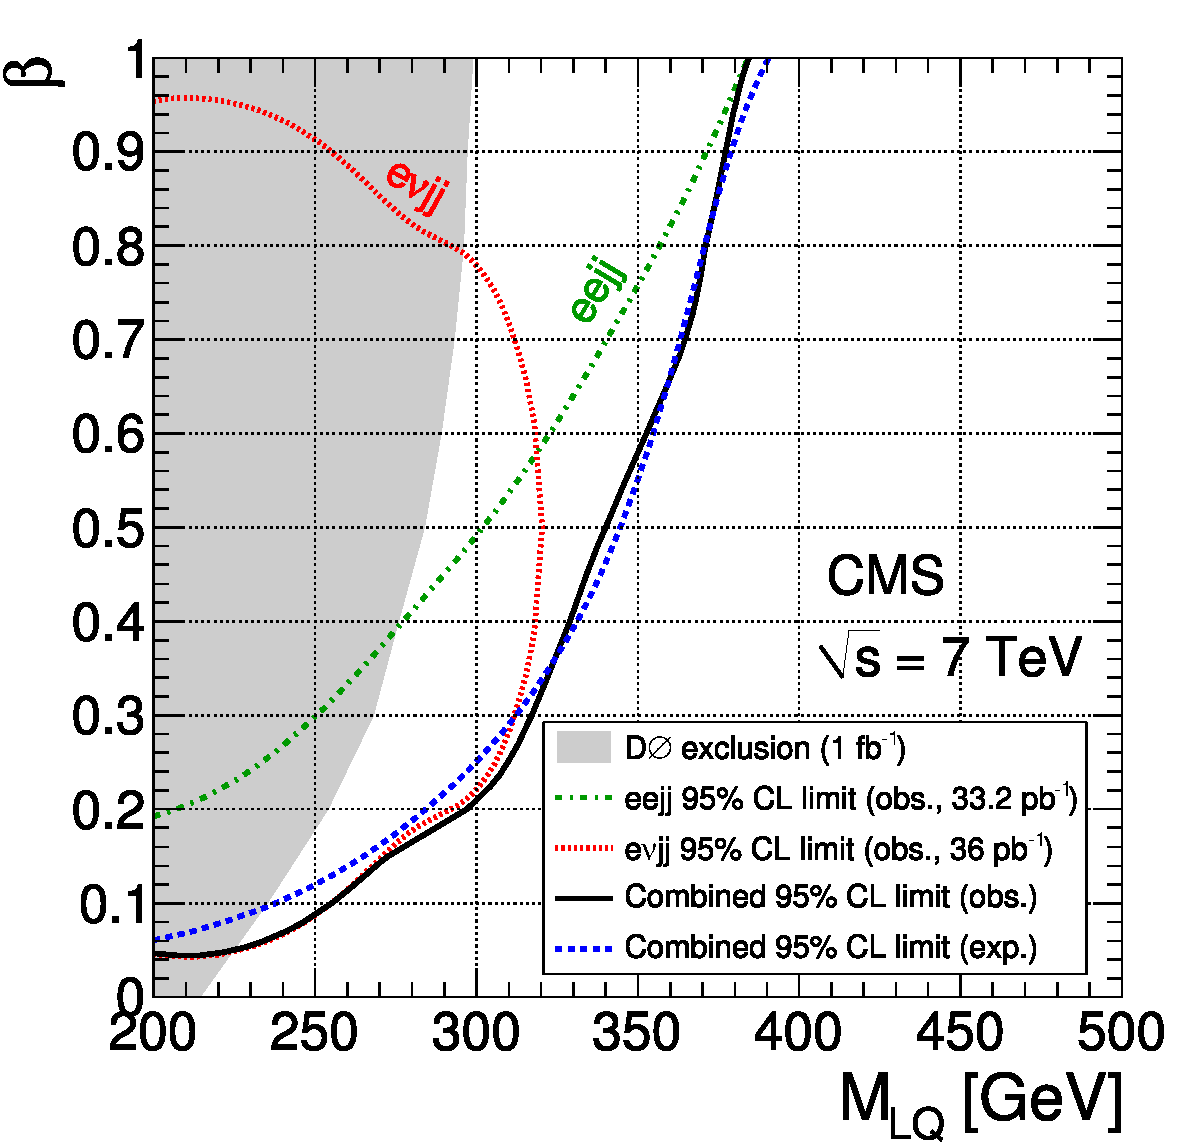
\includegraphics[angle=0]{beta_vs_m_excl_comb.pdf}} &
%      \resizebox{7.9cm}{!}{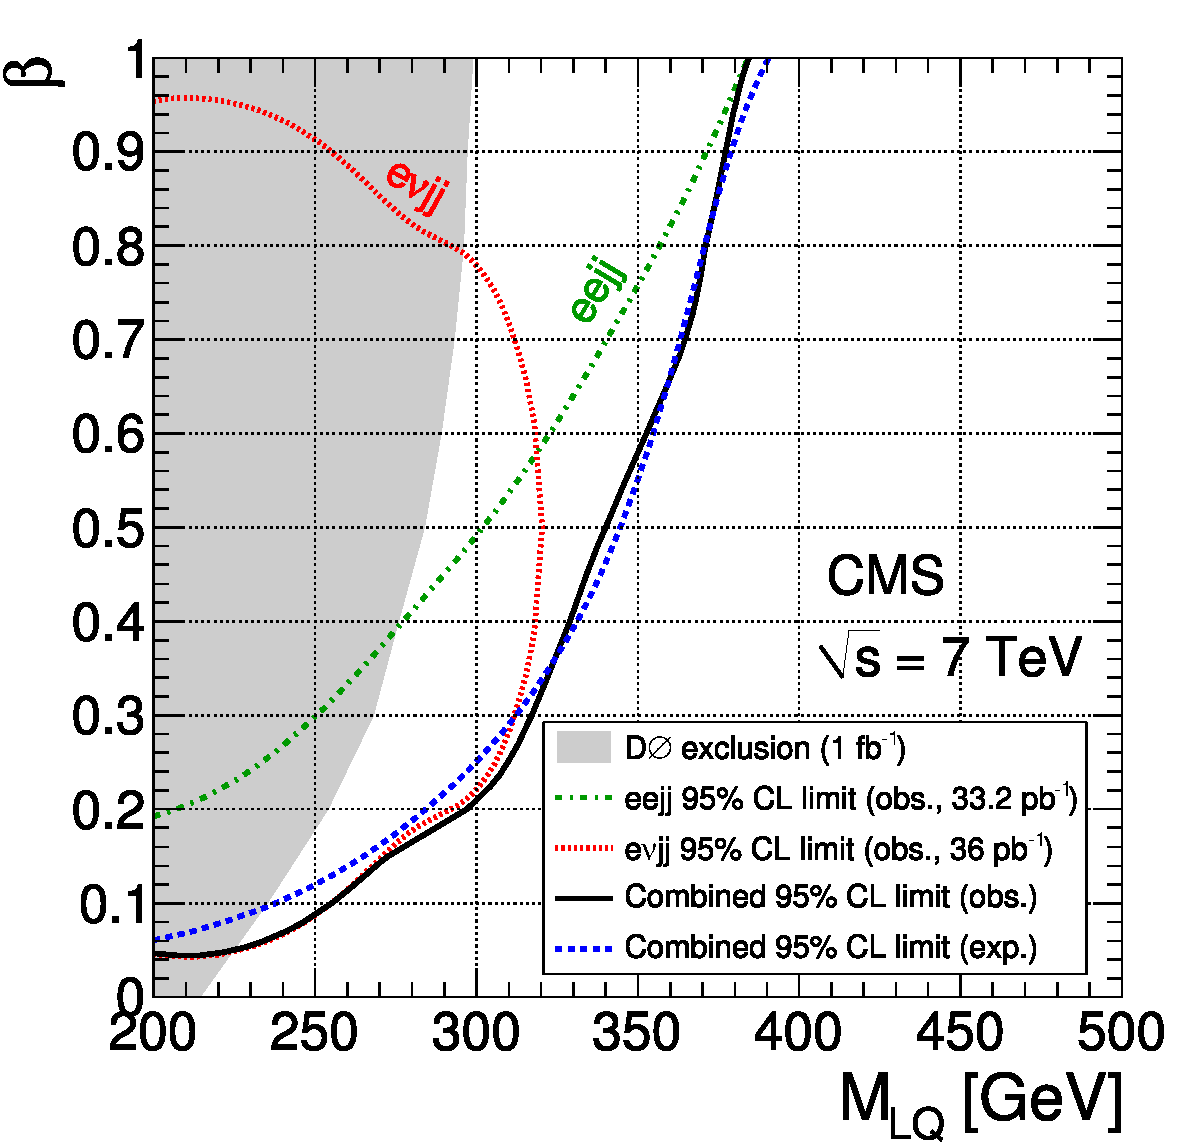
\includegraphics[angle=0]{beta_vs_m_excl_comb.pdf}} \\
    \end{tabular}
    \caption{(Left) Upper limits as a function of resonance mass, on the \Zprime 
cross section relative to standard model Z boson production, obtained combining dielectron and
dimuon final states. (Right) Upper limits as a function of the resonance mass, on the 
\Wprime cross section for the individual electron+neutrino and muon+neutrino channels, 
and their combination.}
    \label{fig:resonances}
  \end{center}
\end{figure}

\section*{Acknowledgments}

\section*{References}
\begin{thebibliography}{99}

\bibitem{CMSJINST}The CMS Collaboration, \Journal{\JINST}{3}{S08004}{2008}.
\bibitem{Chatrchyan:2011wq}The CMS Collaboration, {\em arXiv:1103.0981} (2011). Accepted for publication in \JHEP.
\bibitem{CMSPAS:EXO-10-019}The CMS Collaboration, {\em CMS Physics Analysis Summary} {\bf EXO-10-019} (2011).
\bibitem{Khachatryan201121}The CMS Collaboration, \Journal{\PLB}{698}{21}{2011}.
\bibitem{Chatrchyan:2011dx}The CMS Collaboration, {\em arXiv:1103.0030} (2011). Accepted for publication in \PLB.

%\bibitem{ja}C Jarlskog in {\em CP Violation}, ed. C Jarlskog
%(World Scientific, Singapore, 1988).
%\bibitem{ma}L. Maiani, \Journal{\PLB}{62}{183}{1976}.
%\bibitem{bu}J.D. Bjorken and I. Dunietz, \Journal{\PRD}{36}{2109}{1987}.
%\bibitem{bd}C.D. Buchanan {\it et al}, \Journal{\PRD}{45}{4088}{1992}.

\end{thebibliography}

\end{document}

%%%%%%%%%%%%%%%%%%%%%%
% End of moriond.tex  %
%%%%%%%%%%%%%%%%%%%%%%

